\documentclass[1p]{elsarticle_modified}
%\bibliographystyle{elsarticle-num}

%\usepackage[colorlinks]{hyperref}
%\usepackage{abbrmath_seonhwa} %\Abb, \Ascr, \Acal ,\Abf, \Afrak
\usepackage{amsfonts}
\usepackage{amssymb}
\usepackage{amsmath}
\usepackage{amsthm}
\usepackage{scalefnt}
\usepackage{amsbsy}
\usepackage{kotex}
\usepackage{caption}
\usepackage{subfig}
\usepackage{color}
\usepackage{graphicx}
\usepackage{xcolor} %% white, black, red, green, blue, cyan, magenta, yellow
\usepackage{float}
\usepackage{setspace}
\usepackage{hyperref}

\usepackage{tikz}
\usetikzlibrary{arrows}

\usepackage{multirow}
\usepackage{array} % fixed length table
\usepackage{hhline}

%%%%%%%%%%%%%%%%%%%%%
\makeatletter
\renewcommand*\env@matrix[1][\arraystretch]{%
	\edef\arraystretch{#1}%
	\hskip -\arraycolsep
	\let\@ifnextchar\new@ifnextchar
	\array{*\c@MaxMatrixCols c}}
\makeatother %https://tex.stackexchange.com/questions/14071/how-can-i-increase-the-line-spacing-in-a-matrix
%%%%%%%%%%%%%%%

\usepackage[normalem]{ulem}

\newcommand{\msout}[1]{\ifmmode\text{\sout{\ensuremath{#1}}}\else\sout{#1}\fi}
%SOURCE: \msout is \stkout macro in https://tex.stackexchange.com/questions/20609/strikeout-in-math-mode

\newcommand{\cancel}[1]{
	\ifmmode
	{\color{red}\msout{#1}}
	\else
	{\color{red}\sout{#1}}
	\fi
}

\newcommand{\add}[1]{
	{\color{blue}\uwave{#1}}
}

\newcommand{\replace}[2]{
	\ifmmode
	{\color{red}\msout{#1}}{\color{blue}\uwave{#2}}
	\else
	{\color{red}\sout{#1}}{\color{blue}\uwave{#2}}
	\fi
}

\newcommand{\Sol}{\mathcal{S}} %segment
\newcommand{\D}{D} %diagram
\newcommand{\A}{\mathcal{A}} %arc


%%%%%%%%%%%%%%%%%%%%%%%%%%%%%5 test

\def\sl{\operatorname{\textup{SL}}(2,\Cbb)}
\def\psl{\operatorname{\textup{PSL}}(2,\Cbb)}
\def\quan{\mkern 1mu \triangleright \mkern 1mu}

\theoremstyle{definition}
\newtheorem{thm}{Theorem}[section]
\newtheorem{prop}[thm]{Proposition}
\newtheorem{lem}[thm]{Lemma}
\newtheorem{ques}[thm]{Question}
\newtheorem{cor}[thm]{Corollary}
\newtheorem{defn}[thm]{Definition}
\newtheorem{exam}[thm]{Example}
\newtheorem{rmk}[thm]{Remark}
\newtheorem{alg}[thm]{Algorithm}

\newcommand{\I}{\sqrt{-1}}
\begin{document}

%\begin{frontmatter}
%
%\title{Boundary parabolic representations of knots up to 8 crossings}
%
%%% Group authors per affiliation:
%\author{Yunhi Cho} 
%\address{Department of Mathematics, University of Seoul, Seoul, Korea}
%\ead{yhcho@uos.ac.kr}
%
%
%\author{Seonhwa Kim} %\fnref{s_kim}}
%\address{Center for Geometry and Physics, Institute for Basic Science, Pohang, 37673, Korea}
%\ead{ryeona17@ibs.re.kr}
%
%\author{Hyuk Kim}
%\address{Department of Mathematical Sciences, Seoul National University, Seoul 08826, Korea}
%\ead{hyukkim@snu.ac.kr}
%
%\author{Seokbeom Yoon}
%\address{Department of Mathematical Sciences, Seoul National University, Seoul, 08826,  Korea}
%\ead{sbyoon15@snu.ac.kr}
%
%\begin{abstract}
%We find all boundary parabolic representation of knots up to 8 crossings.
%
%\end{abstract}
%\begin{keyword}
%    \MSC[2010] 57M25 
%\end{keyword}
%
%\end{frontmatter}

%\linenumbers
%\tableofcontents
%
\newcommand\colored[1]{\textcolor{white}{\rule[-0.35ex]{0.8em}{1.4ex}}\kern-0.8em\color{red} #1}%
%\newcommand\colored[1]{\textcolor{white}{ #1}\kern-2.17ex	\textcolor{white}{ #1}\kern-1.81ex	\textcolor{white}{ #1}\kern-2.15ex\color{red}#1	}

{\Large $\underline{12a_{0927}~(K12a_{0927})}$}

\setlength{\tabcolsep}{10pt}
\renewcommand{\arraystretch}{1.6}
\vspace{1cm}\begin{tabular}{m{100pt}>{\centering\arraybackslash}m{274pt}}
\multirow{5}{120pt}{
	\centering
	\includegraphics[width=112pt]{../../../GIT/diagram.site/Diagrams/png/1728_12a_0927.png}\\
\ \ \ A knot diagram\footnotemark}&
\allowdisplaybreaks
\textbf{Linearized knot diagam} \\
\cline{2-2}
 &
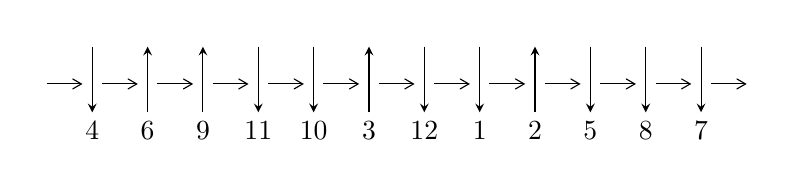
\begin{tikzpicture}[x=20pt, y=17pt]
	% nodes
	\node (C0) at (0, 0) {};
	\node (C1) at (1, 0) {};
	\node (C1U) at (1, +1) {};
	\node (C1D) at (1, -1) {4};

	\node (C2) at (2, 0) {};
	\node (C2U) at (2, +1) {};
	\node (C2D) at (2, -1) {6};

	\node (C3) at (3, 0) {};
	\node (C3U) at (3, +1) {};
	\node (C3D) at (3, -1) {9};

	\node (C4) at (4, 0) {};
	\node (C4U) at (4, +1) {};
	\node (C4D) at (4, -1) {11};

	\node (C5) at (5, 0) {};
	\node (C5U) at (5, +1) {};
	\node (C5D) at (5, -1) {10};

	\node (C6) at (6, 0) {};
	\node (C6U) at (6, +1) {};
	\node (C6D) at (6, -1) {3};

	\node (C7) at (7, 0) {};
	\node (C7U) at (7, +1) {};
	\node (C7D) at (7, -1) {12};

	\node (C8) at (8, 0) {};
	\node (C8U) at (8, +1) {};
	\node (C8D) at (8, -1) {1};

	\node (C9) at (9, 0) {};
	\node (C9U) at (9, +1) {};
	\node (C9D) at (9, -1) {2};

	\node (C10) at (10, 0) {};
	\node (C10U) at (10, +1) {};
	\node (C10D) at (10, -1) {5};

	\node (C11) at (11, 0) {};
	\node (C11U) at (11, +1) {};
	\node (C11D) at (11, -1) {8};

	\node (C12) at (12, 0) {};
	\node (C12U) at (12, +1) {};
	\node (C12D) at (12, -1) {7};
	\node (C13) at (13, 0) {};

	% arrows
	\draw[->,>={angle 60}]
	(C0) edge (C1) (C1) edge (C2) (C2) edge (C3) (C3) edge (C4) (C4) edge (C5) (C5) edge (C6) (C6) edge (C7) (C7) edge (C8) (C8) edge (C9) (C9) edge (C10) (C10) edge (C11) (C11) edge (C12) (C12) edge (C13) ;	\draw[->,>=stealth]
	(C1U) edge (C1D) (C2D) edge (C2U) (C3D) edge (C3U) (C4U) edge (C4D) (C5U) edge (C5D) (C6D) edge (C6U) (C7U) edge (C7D) (C8U) edge (C8D) (C9D) edge (C9U) (C10U) edge (C10D) (C11U) edge (C11D) (C12U) edge (C12D) ;
	\end{tikzpicture} \\
\hhline{~~} \\& 
\textbf{Solving Sequence} \\ \cline{2-2} 
 &
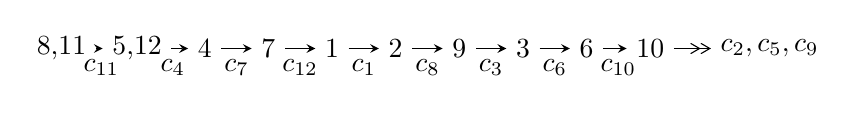
\begin{tikzpicture}[x=23pt, y=7pt]
	% node
	\node (A0) at (-1/8, 0) {8,11};
	\node (A1) at (17/16, 0) {5,12};
	\node (A2) at (17/8, 0) {4};
	\node (A3) at (25/8, 0) {7};
	\node (A4) at (33/8, 0) {1};
	\node (A5) at (41/8, 0) {2};
	\node (A6) at (49/8, 0) {9};
	\node (A7) at (57/8, 0) {3};
	\node (A8) at (65/8, 0) {6};
	\node (A9) at (73/8, 0) {10};
	\node (C1) at (1/2, -1) {$c_{11}$};
	\node (C2) at (13/8, -1) {$c_{4}$};
	\node (C3) at (21/8, -1) {$c_{7}$};
	\node (C4) at (29/8, -1) {$c_{12}$};
	\node (C5) at (37/8, -1) {$c_{1}$};
	\node (C6) at (45/8, -1) {$c_{8}$};
	\node (C7) at (53/8, -1) {$c_{3}$};
	\node (C8) at (61/8, -1) {$c_{6}$};
	\node (C9) at (69/8, -1) {$c_{10}$};
	\node (A10) at (11, 0) {$c_{2},c_{5},c_{9}$};

	% edge
	\draw[->,>=stealth]	
	(A0) edge (A1) (A1) edge (A2) (A2) edge (A3) (A3) edge (A4) (A4) edge (A5) (A5) edge (A6) (A6) edge (A7) (A7) edge (A8) (A8) edge (A9) ;
	\draw[->>,>={angle 60}]	
	(A9) edge (A10);
\end{tikzpicture} \\ 

\end{tabular} \\

\footnotetext{
The image of knot diagram is generated by the software ``\textbf{Draw programme}" developed by Andrew Bartholomew(\url{http://www.layer8.co.uk/maths/draw/index.htm\#Running-draw}), where we modified some parts for our purpose(\url{https://github.com/CATsTAILs/LinksPainter}).
}\phantom \\ \newline 
\centering \textbf{Ideals for irreducible components\footnotemark of $X_{\text{par}}$} 
 
\begin{align*}
I^u_{1}&=\langle 
1.17204\times10^{92} u^{100}+5.80593\times10^{92} u^{99}+\cdots+1.37181\times10^{93} b-1.38998\times10^{93},\\
\phantom{I^u_{1}}&\phantom{= \langle  }1.34846\times10^{94} u^{100}+5.39689\times10^{93} u^{99}+\cdots+9.60265\times10^{93} a+1.74373\times10^{94},\;u^{101}+46 u^{99}+\cdots+u-1\rangle \\
I^u_{2}&=\langle 
- u^{18}- u^{17}+\cdots+b+2 u,\;u^{18}+3 u^{17}+\cdots+a-3,\;u^{19}- u^{18}+\cdots-2 u+1\rangle \\
\\
\end{align*}
\raggedright * 2 irreducible components of $\dim_{\mathbb{C}}=0$, with total 120 representations.\\
\footnotetext{All coefficients of polynomials are rational numbers. But the coefficients are sometimes approximated in decimal forms when there is not enough margin.}
\newpage
\renewcommand{\arraystretch}{1}
\centering \section*{I. $I^u_{1}= \langle 1.17\times10^{92} u^{100}+5.81\times10^{92} u^{99}+\cdots+1.37\times10^{93} b-1.39\times10^{93},\;1.35\times10^{94} u^{100}+5.40\times10^{93} u^{99}+\cdots+9.60\times10^{93} a+1.74\times10^{94},\;u^{101}+46 u^{99}+\cdots+u-1 \rangle$}
\flushleft \textbf{(i) Arc colorings}\\
\begin{tabular}{m{7pt} m{180pt} m{7pt} m{180pt} }
\flushright $a_{8}=$&$\begin{pmatrix}0\\u\end{pmatrix}$ \\
\flushright $a_{11}=$&$\begin{pmatrix}1\\0\end{pmatrix}$ \\
\flushright $a_{5}=$&$\begin{pmatrix}-1.40425 u^{100}-0.562021 u^{99}+\cdots-10.2436 u-1.81588\\-0.0854374 u^{100}-0.423232 u^{99}+\cdots-1.90512 u+1.01325\end{pmatrix}$ \\
\flushright $a_{12}=$&$\begin{pmatrix}1\\u^2\end{pmatrix}$ \\
\flushright $a_{4}=$&$\begin{pmatrix}-1.48969 u^{100}-0.985252 u^{99}+\cdots-12.1487 u-0.802639\\-0.0854374 u^{100}-0.423232 u^{99}+\cdots-1.90512 u+1.01325\end{pmatrix}$ \\
\flushright $a_{7}=$&$\begin{pmatrix}u\\u^3+u\end{pmatrix}$ \\
\flushright $a_{1}=$&$\begin{pmatrix}u^2+1\\u^4+2 u^2\end{pmatrix}$ \\
\flushright $a_{2}=$&$\begin{pmatrix}-0.940964 u^{100}-0.279768 u^{99}+\cdots-5.22472 u-1.91292\\-0.237618 u^{100}-0.171606 u^{99}+\cdots-0.697920 u+0.894695\end{pmatrix}$ \\
\flushright $a_{9}=$&$\begin{pmatrix}- u^5-2 u^3- u\\- u^7-3 u^5-2 u^3+u\end{pmatrix}$ \\
\flushright $a_{3}=$&$\begin{pmatrix}-1.29125 u^{100}-0.629929 u^{99}+\cdots-11.0393 u-0.969058\\-0.132061 u^{100}-0.130376 u^{99}+\cdots-2.32353 u+0.594206\end{pmatrix}$ \\
\flushright $a_{6}=$&$\begin{pmatrix}-0.868953 u^{100}+1.16462 u^{99}+\cdots-14.5751 u-2.32310\\0.206049 u^{100}-0.125342 u^{99}+\cdots-0.0119723 u+0.0903791\end{pmatrix}$ \\
\flushright $a_{10}=$&$\begin{pmatrix}0.482166 u^{100}+1.70715 u^{99}+\cdots+4.91113 u+0.887370\\-0.114195 u^{100}-0.653840 u^{99}+\cdots-0.298804 u+0.247379\end{pmatrix}$\\&\end{tabular}
\flushleft \textbf{(ii) Obstruction class $= -1$}\\~\\
\flushleft \textbf{(iii) Cusp Shapes $= 2.59770 u^{100}-1.50889 u^{99}+\cdots+12.8990 u+3.67843$}\\~\\
\newpage\renewcommand{\arraystretch}{1}
\flushleft \textbf{(iv) u-Polynomials at the component}\newline \\
\begin{tabular}{m{50pt}|m{274pt}}
Crossings & \hspace{64pt}u-Polynomials at each crossing \\
\hline $$\begin{aligned}c_{1}\end{aligned}$$&$\begin{aligned}
&u^{101}-17 u^{100}+\cdots+59829 u-3461
\end{aligned}$\\
\hline $$\begin{aligned}c_{2},c_{6}\end{aligned}$$&$\begin{aligned}
&u^{101}+2 u^{100}+\cdots+9256 u-1034
\end{aligned}$\\
\hline $$\begin{aligned}c_{3}\end{aligned}$$&$\begin{aligned}
&u^{101}- u^{100}+\cdots-91 u+1
\end{aligned}$\\
\hline $$\begin{aligned}c_{4},c_{5},c_{10}\end{aligned}$$&$\begin{aligned}
&u^{101}- u^{100}+\cdots+22 u-4
\end{aligned}$\\
\hline $$\begin{aligned}c_{7},c_{11},c_{12}\end{aligned}$$&$\begin{aligned}
&u^{101}+46 u^{99}+\cdots+u-1
\end{aligned}$\\
\hline $$\begin{aligned}c_{8}\end{aligned}$$&$\begin{aligned}
&u^{101}-2 u^{99}+\cdots+712 u-232
\end{aligned}$\\
\hline $$\begin{aligned}c_{9}\end{aligned}$$&$\begin{aligned}
&u^{101}+3 u^{100}+\cdots+5282083 u+2372859
\end{aligned}$\\
\hline
\end{tabular}\\~\\
\newpage\renewcommand{\arraystretch}{1}
\flushleft \textbf{(v) Riley Polynomials at the component}\newline \\
\begin{tabular}{m{50pt}|m{274pt}}
Crossings & \hspace{64pt}Riley Polynomials at each crossing \\
\hline $$\begin{aligned}c_{1}\end{aligned}$$&$\begin{aligned}
&y^{101}+15 y^{100}+\cdots+43620123 y-11978521
\end{aligned}$\\
\hline $$\begin{aligned}c_{2},c_{6}\end{aligned}$$&$\begin{aligned}
&y^{101}-84 y^{100}+\cdots+41122612 y-1069156
\end{aligned}$\\
\hline $$\begin{aligned}c_{3}\end{aligned}$$&$\begin{aligned}
&y^{101}-9 y^{100}+\cdots+7531 y-1
\end{aligned}$\\
\hline $$\begin{aligned}c_{4},c_{5},c_{10}\end{aligned}$$&$\begin{aligned}
&y^{101}+107 y^{100}+\cdots-708 y-16
\end{aligned}$\\
\hline $$\begin{aligned}c_{7},c_{11},c_{12}\end{aligned}$$&$\begin{aligned}
&y^{101}+92 y^{100}+\cdots+19 y-1
\end{aligned}$\\
\hline $$\begin{aligned}c_{8}\end{aligned}$$&$\begin{aligned}
&y^{101}-4 y^{100}+\cdots+171472 y-53824
\end{aligned}$\\
\hline $$\begin{aligned}c_{9}\end{aligned}$$&$\begin{aligned}
&y^{101}-39 y^{100}+\cdots+211509629585425 y-5630459833881
\end{aligned}$\\
\hline
\end{tabular}\\~\\
\newpage\flushleft \textbf{(vi) Complex Volumes and Cusp Shapes}
$$\begin{array}{c|c|c}  
\text{Solutions to }I^u_{1}& \I (\text{vol} + \sqrt{-1}CS) & \text{Cusp shape}\\
 \hline 
\begin{aligned}
u &= \phantom{-}0.338601 + 0.929957 I \\
a &= -0.796464 + 1.012730 I \\
b &= -0.022504 - 1.387680 I\end{aligned}
 & \phantom{-}5.03799 - 2.07046 I & \phantom{-0.000000 } 0 \\ \hline\begin{aligned}
u &= \phantom{-}0.338601 - 0.929957 I \\
a &= -0.796464 - 1.012730 I \\
b &= -0.022504 + 1.387680 I\end{aligned}
 & \phantom{-}5.03799 + 2.07046 I & \phantom{-0.000000 } 0 \\ \hline\begin{aligned}
u &= \phantom{-}0.813138 + 0.514209 I \\
a &= \phantom{-}0.90012 - 1.28023 I \\
b &= \phantom{-}0.02602 + 1.43752 I\end{aligned}
 & \phantom{-}4.47550 - 2.65435 I & \phantom{-0.000000 } 0 \\ \hline\begin{aligned}
u &= \phantom{-}0.813138 - 0.514209 I \\
a &= \phantom{-}0.90012 + 1.28023 I \\
b &= \phantom{-}0.02602 - 1.43752 I\end{aligned}
 & \phantom{-}4.47550 + 2.65435 I & \phantom{-0.000000 } 0 \\ \hline\begin{aligned}
u &= -0.560557 + 0.768072 I \\
a &= -0.421182 - 1.247580 I \\
b &= \phantom{-}0.25302 + 1.54034 I\end{aligned}
 & \phantom{-}9.75188 - 8.20632 I & \phantom{-0.000000 } 0 \\ \hline\begin{aligned}
u &= -0.560557 - 0.768072 I \\
a &= -0.421182 + 1.247580 I \\
b &= \phantom{-}0.25302 - 1.54034 I\end{aligned}
 & \phantom{-}9.75188 + 8.20632 I & \phantom{-0.000000 } 0 \\ \hline\begin{aligned}
u &= \phantom{-}0.128473 + 1.056460 I \\
a &= -0.503339 + 0.351516 I \\
b &= -0.444666 + 0.213037 I\end{aligned}
 & -0.200435 + 0.703668 I & \phantom{-0.000000 } 0 \\ \hline\begin{aligned}
u &= \phantom{-}0.128473 - 1.056460 I \\
a &= -0.503339 - 0.351516 I \\
b &= -0.444666 - 0.213037 I\end{aligned}
 & -0.200435 - 0.703668 I & \phantom{-0.000000 } 0 \\ \hline\begin{aligned}
u &= -0.055755 + 1.087090 I \\
a &= \phantom{-}0.269569 + 1.352040 I \\
b &= \phantom{-}0.645189 - 0.746095 I\end{aligned}
 & \phantom{-}3.31819 + 0.06863 I & \phantom{-0.000000 } 0 \\ \hline\begin{aligned}
u &= -0.055755 - 1.087090 I \\
a &= \phantom{-}0.269569 - 1.352040 I \\
b &= \phantom{-}0.645189 + 0.746095 I\end{aligned}
 & \phantom{-}3.31819 - 0.06863 I & \phantom{-0.000000 } 0\\
 \hline 
 \end{array}$$\newpage$$\begin{array}{c|c|c}  
\text{Solutions to }I^u_{1}& \I (\text{vol} + \sqrt{-1}CS) & \text{Cusp shape}\\
 \hline 
\begin{aligned}
u &= -0.321913 + 0.829241 I \\
a &= -0.045721 + 1.039040 I \\
b &= -0.10695 - 1.44066 I\end{aligned}
 & \phantom{-}5.22244 - 2.50144 I & \phantom{-0.000000 } 0 \\ \hline\begin{aligned}
u &= -0.321913 - 0.829241 I \\
a &= -0.045721 - 1.039040 I \\
b &= -0.10695 + 1.44066 I\end{aligned}
 & \phantom{-}5.22244 + 2.50144 I & \phantom{-0.000000 } 0 \\ \hline\begin{aligned}
u &= \phantom{-}0.406936 + 0.775815 I \\
a &= -0.300390 - 0.045936 I \\
b &= \phantom{-}0.734298 - 0.534377 I\end{aligned}
 & \phantom{-}2.94013 + 4.57156 I & \phantom{-0.000000 } 0 \\ \hline\begin{aligned}
u &= \phantom{-}0.406936 - 0.775815 I \\
a &= -0.300390 + 0.045936 I \\
b &= \phantom{-}0.734298 + 0.534377 I\end{aligned}
 & \phantom{-}2.94013 - 4.57156 I & \phantom{-0.000000 } 0 \\ \hline\begin{aligned}
u &= \phantom{-}0.787460 + 0.379801 I \\
a &= -0.855942 + 0.809852 I \\
b &= -0.140540 - 1.265200 I\end{aligned}
 & \phantom{-}2.64686 - 2.47490 I & \phantom{-0.000000 } 0 \\ \hline\begin{aligned}
u &= \phantom{-}0.787460 - 0.379801 I \\
a &= -0.855942 - 0.809852 I \\
b &= -0.140540 + 1.265200 I\end{aligned}
 & \phantom{-}2.64686 + 2.47490 I & \phantom{-0.000000 } 0 \\ \hline\begin{aligned}
u &= -0.345176 + 1.073310 I \\
a &= -0.012039 + 0.367281 I \\
b &= \phantom{-}0.639537 - 0.260559 I\end{aligned}
 & \phantom{-}2.13144 + 4.10343 I & \phantom{-0.000000 } 0 \\ \hline\begin{aligned}
u &= -0.345176 - 1.073310 I \\
a &= -0.012039 - 0.367281 I \\
b &= \phantom{-}0.639537 + 0.260559 I\end{aligned}
 & \phantom{-}2.13144 - 4.10343 I & \phantom{-0.000000 } 0 \\ \hline\begin{aligned}
u &= \phantom{-}0.844506 + 0.188748 I \\
a &= -0.535125 + 0.252887 I \\
b &= -0.087205 - 1.339120 I\end{aligned}
 & \phantom{-}2.69324 - 2.22762 I & \phantom{-0.000000 } 0 \\ \hline\begin{aligned}
u &= \phantom{-}0.844506 - 0.188748 I \\
a &= -0.535125 - 0.252887 I \\
b &= -0.087205 + 1.339120 I\end{aligned}
 & \phantom{-}2.69324 + 2.22762 I & \phantom{-0.000000 } 0\\
 \hline 
 \end{array}$$\newpage$$\begin{array}{c|c|c}  
\text{Solutions to }I^u_{1}& \I (\text{vol} + \sqrt{-1}CS) & \text{Cusp shape}\\
 \hline 
\begin{aligned}
u &= -0.799774 + 0.329138 I \\
a &= -1.54547 - 0.83395 I \\
b &= -0.28641 + 1.56866 I\end{aligned}
 & \phantom{-}8.3431 + 12.9028 I & \phantom{-0.000000 } 0. - 7.85868 I \\ \hline\begin{aligned}
u &= -0.799774 - 0.329138 I \\
a &= -1.54547 + 0.83395 I \\
b &= -0.28641 - 1.56866 I\end{aligned}
 & \phantom{-}8.3431 - 12.9028 I & \phantom{-0.000000 -}0. + 7.85868 I \\ \hline\begin{aligned}
u &= -0.732389 + 0.383945 I \\
a &= \phantom{-}0.303247 + 0.402040 I \\
b &= \phantom{-}0.127737 - 0.125151 I\end{aligned}
 & -0.84943 + 2.18733 I & -11.7134 - 11.9875 I \\ \hline\begin{aligned}
u &= -0.732389 - 0.383945 I \\
a &= \phantom{-}0.303247 - 0.402040 I \\
b &= \phantom{-}0.127737 + 0.125151 I\end{aligned}
 & -0.84943 - 2.18733 I & -11.7134 + 11.9875 I \\ \hline\begin{aligned}
u &= \phantom{-}0.754882 + 0.273496 I \\
a &= -0.956345 + 0.605149 I \\
b &= -0.846330 - 0.599759 I\end{aligned}
 & \phantom{-}1.25837 - 8.74577 I & -2.71147 + 8.57986 I \\ \hline\begin{aligned}
u &= \phantom{-}0.754882 - 0.273496 I \\
a &= -0.956345 - 0.605149 I \\
b &= -0.846330 + 0.599759 I\end{aligned}
 & \phantom{-}1.25837 + 8.74577 I & -2.71147 - 8.57986 I \\ \hline\begin{aligned}
u &= -0.742037 + 0.242897 I \\
a &= \phantom{-}1.91043 + 0.22567 I \\
b &= \phantom{-}0.16250 - 1.46227 I\end{aligned}
 & \phantom{-}3.30401 + 6.47041 I & -1.74126 - 7.20929 I \\ \hline\begin{aligned}
u &= -0.742037 - 0.242897 I \\
a &= \phantom{-}1.91043 - 0.22567 I \\
b &= \phantom{-}0.16250 + 1.46227 I\end{aligned}
 & \phantom{-}3.30401 - 6.47041 I & -1.74126 + 7.20929 I \\ \hline\begin{aligned}
u &= -0.777007\phantom{ +0.000000I} \\
a &= -0.409554\phantom{ +0.000000I} \\
b &= -0.578616\phantom{ +0.000000I}\end{aligned}
 & -1.11245\phantom{ +0.000000I} & -11.1750\phantom{ +0.000000I} \\ \hline\begin{aligned}
u &= -0.025748 + 1.236330 I \\
a &= \phantom{-}0.824447 - 0.076392 I \\
b &= -0.179975 + 1.350560 I\end{aligned}
 & \phantom{-}10.93490 + 2.78038 I & \phantom{-0.000000 } 0\\
 \hline 
 \end{array}$$\newpage$$\begin{array}{c|c|c}  
\text{Solutions to }I^u_{1}& \I (\text{vol} + \sqrt{-1}CS) & \text{Cusp shape}\\
 \hline 
\begin{aligned}
u &= -0.025748 - 1.236330 I \\
a &= \phantom{-}0.824447 + 0.076392 I \\
b &= -0.179975 - 1.350560 I\end{aligned}
 & \phantom{-}10.93490 - 2.78038 I & \phantom{-0.000000 } 0 \\ \hline\begin{aligned}
u &= -0.159559 + 1.251210 I \\
a &= -1.43728 - 1.79915 I \\
b &= -0.266877 + 1.026130 I\end{aligned}
 & \phantom{-}2.17976 + 1.85998 I & \phantom{-0.000000 } 0 \\ \hline\begin{aligned}
u &= -0.159559 - 1.251210 I \\
a &= -1.43728 + 1.79915 I \\
b &= -0.266877 - 1.026130 I\end{aligned}
 & \phantom{-}2.17976 - 1.85998 I & \phantom{-0.000000 } 0 \\ \hline\begin{aligned}
u &= \phantom{-}0.681119 + 0.191835 I \\
a &= \phantom{-}1.338130 - 0.230387 I \\
b &= \phantom{-}0.557811 + 0.339618 I\end{aligned}
 & -2.58528 - 3.94320 I & -8.28628 + 7.57752 I \\ \hline\begin{aligned}
u &= \phantom{-}0.681119 - 0.191835 I \\
a &= \phantom{-}1.338130 + 0.230387 I \\
b &= \phantom{-}0.557811 - 0.339618 I\end{aligned}
 & -2.58528 + 3.94320 I & -8.28628 - 7.57752 I \\ \hline\begin{aligned}
u &= -0.659379 + 0.224660 I \\
a &= -0.421405 - 0.382008 I \\
b &= -0.933561 - 0.630970 I\end{aligned}
 & \phantom{-}1.19502 + 2.86675 I & -0.48560 - 5.63717 I \\ \hline\begin{aligned}
u &= -0.659379 - 0.224660 I \\
a &= -0.421405 + 0.382008 I \\
b &= -0.933561 + 0.630970 I\end{aligned}
 & \phantom{-}1.19502 - 2.86675 I & -0.48560 + 5.63717 I \\ \hline\begin{aligned}
u &= \phantom{-}0.123790 + 1.319540 I \\
a &= -0.028371 + 1.029170 I \\
b &= \phantom{-}0.419572 - 0.634578 I\end{aligned}
 & \phantom{-}4.45606 + 0.45152 I & \phantom{-0.000000 } 0 \\ \hline\begin{aligned}
u &= \phantom{-}0.123790 - 1.319540 I \\
a &= -0.028371 - 1.029170 I \\
b &= \phantom{-}0.419572 + 0.634578 I\end{aligned}
 & \phantom{-}4.45606 - 0.45152 I & \phantom{-0.000000 } 0 \\ \hline\begin{aligned}
u &= -0.048734 + 1.338630 I \\
a &= \phantom{-}0.55365 - 2.90345 I \\
b &= \phantom{-}0.09844 + 1.58170 I\end{aligned}
 & \phantom{-}11.89780 - 2.24580 I & \phantom{-0.000000 } 0\\
 \hline 
 \end{array}$$\newpage$$\begin{array}{c|c|c}  
\text{Solutions to }I^u_{1}& \I (\text{vol} + \sqrt{-1}CS) & \text{Cusp shape}\\
 \hline 
\begin{aligned}
u &= -0.048734 - 1.338630 I \\
a &= \phantom{-}0.55365 + 2.90345 I \\
b &= \phantom{-}0.09844 - 1.58170 I\end{aligned}
 & \phantom{-}11.89780 + 2.24580 I & \phantom{-0.000000 } 0 \\ \hline\begin{aligned}
u &= \phantom{-}0.452314 + 1.270540 I \\
a &= \phantom{-}0.78602 - 1.48254 I \\
b &= \phantom{-}0.167551 + 1.383620 I\end{aligned}
 & \phantom{-}7.24145 - 6.94635 I & \phantom{-0.000000 } 0 \\ \hline\begin{aligned}
u &= \phantom{-}0.452314 - 1.270540 I \\
a &= \phantom{-}0.78602 + 1.48254 I \\
b &= \phantom{-}0.167551 - 1.383620 I\end{aligned}
 & \phantom{-}7.24145 + 6.94635 I & \phantom{-0.000000 } 0 \\ \hline\begin{aligned}
u &= -0.238627 + 1.333130 I \\
a &= \phantom{-}0.079299 + 0.683567 I \\
b &= \phantom{-}0.655029 - 0.237112 I\end{aligned}
 & \phantom{-}3.08685 + 3.11452 I & \phantom{-0.000000 } 0 \\ \hline\begin{aligned}
u &= -0.238627 - 1.333130 I \\
a &= \phantom{-}0.079299 - 0.683567 I \\
b &= \phantom{-}0.655029 + 0.237112 I\end{aligned}
 & \phantom{-}3.08685 - 3.11452 I & \phantom{-0.000000 } 0 \\ \hline\begin{aligned}
u &= \phantom{-}0.608901 + 0.192542 I \\
a &= -0.385198 + 1.115390 I \\
b &= -0.203404 - 0.637908 I\end{aligned}
 & \phantom{-}1.37542 - 2.38581 I & \phantom{-}0.25318 + 6.68724 I \\ \hline\begin{aligned}
u &= \phantom{-}0.608901 - 0.192542 I \\
a &= -0.385198 - 1.115390 I \\
b &= -0.203404 + 0.637908 I\end{aligned}
 & \phantom{-}1.37542 + 2.38581 I & \phantom{-}0.25318 - 6.68724 I \\ \hline\begin{aligned}
u &= -0.212837 + 1.348630 I \\
a &= \phantom{-}0.173204 + 0.342037 I \\
b &= -0.515624 - 0.729139 I\end{aligned}
 & \phantom{-}3.32479 + 3.40667 I & \phantom{-0.000000 } 0 \\ \hline\begin{aligned}
u &= -0.212837 - 1.348630 I \\
a &= \phantom{-}0.173204 - 0.342037 I \\
b &= -0.515624 + 0.729139 I\end{aligned}
 & \phantom{-}3.32479 - 3.40667 I & \phantom{-0.000000 } 0 \\ \hline\begin{aligned}
u &= -0.629319\phantom{ +0.000000I} \\
a &= -0.702050\phantom{ +0.000000I} \\
b &= -0.548156\phantom{ +0.000000I}\end{aligned}
 & -1.22681\phantom{ +0.000000I} & -8.76370\phantom{ +0.000000I}\\
 \hline 
 \end{array}$$\newpage$$\begin{array}{c|c|c}  
\text{Solutions to }I^u_{1}& \I (\text{vol} + \sqrt{-1}CS) & \text{Cusp shape}\\
 \hline 
\begin{aligned}
u &= \phantom{-}0.160524 + 1.364360 I \\
a &= \phantom{-}1.76789 - 1.18203 I \\
b &= -0.009637 + 0.248297 I\end{aligned}
 & \phantom{-}7.62385 - 1.80031 I & \phantom{-0.000000 } 0 \\ \hline\begin{aligned}
u &= \phantom{-}0.160524 - 1.364360 I \\
a &= \phantom{-}1.76789 + 1.18203 I \\
b &= -0.009637 - 0.248297 I\end{aligned}
 & \phantom{-}7.62385 + 1.80031 I & \phantom{-0.000000 } 0 \\ \hline\begin{aligned}
u &= \phantom{-}0.551646 + 0.273553 I \\
a &= \phantom{-}2.47112 - 0.13182 I \\
b &= \phantom{-}0.33166 + 1.54527 I\end{aligned}
 & \phantom{-}8.78897 - 4.29126 I & \phantom{-}1.52859 + 7.08794 I \\ \hline\begin{aligned}
u &= \phantom{-}0.551646 - 0.273553 I \\
a &= \phantom{-}2.47112 + 0.13182 I \\
b &= \phantom{-}0.33166 - 1.54527 I\end{aligned}
 & \phantom{-}8.78897 + 4.29126 I & \phantom{-}1.52859 - 7.08794 I \\ \hline\begin{aligned}
u &= \phantom{-}0.030644 + 1.385460 I \\
a &= \phantom{-}0.44733 - 2.69168 I \\
b &= \phantom{-}0.04203 + 1.58721 I\end{aligned}
 & \phantom{-}11.97780 - 2.24521 I & \phantom{-0.000000 } 0 \\ \hline\begin{aligned}
u &= \phantom{-}0.030644 - 1.385460 I \\
a &= \phantom{-}0.44733 + 2.69168 I \\
b &= \phantom{-}0.04203 - 1.58721 I\end{aligned}
 & \phantom{-}11.97780 + 2.24521 I & \phantom{-0.000000 } 0 \\ \hline\begin{aligned}
u &= -0.151276 + 1.377880 I \\
a &= \phantom{-}0.125296 - 1.287730 I \\
b &= -1.080770 + 0.264270 I\end{aligned}
 & \phantom{-}7.92835 + 1.55973 I & \phantom{-0.000000 } 0 \\ \hline\begin{aligned}
u &= -0.151276 - 1.377880 I \\
a &= \phantom{-}0.125296 + 1.287730 I \\
b &= -1.080770 - 0.264270 I\end{aligned}
 & \phantom{-}7.92835 - 1.55973 I & \phantom{-0.000000 } 0 \\ \hline\begin{aligned}
u &= \phantom{-}0.250853 + 1.369630 I \\
a &= \phantom{-}0.06598 - 1.62169 I \\
b &= \phantom{-}0.055380 + 0.653130 I\end{aligned}
 & \phantom{-}6.32441 - 5.55834 I & \phantom{-0.000000 } 0 \\ \hline\begin{aligned}
u &= \phantom{-}0.250853 - 1.369630 I \\
a &= \phantom{-}0.06598 + 1.62169 I \\
b &= \phantom{-}0.055380 - 0.653130 I\end{aligned}
 & \phantom{-}6.32441 + 5.55834 I & \phantom{-0.000000 } 0\\
 \hline 
 \end{array}$$\newpage$$\begin{array}{c|c|c}  
\text{Solutions to }I^u_{1}& \I (\text{vol} + \sqrt{-1}CS) & \text{Cusp shape}\\
 \hline 
\begin{aligned}
u &= \phantom{-}0.270313 + 1.372210 I \\
a &= -0.659965 + 0.973165 I \\
b &= -0.619046 - 0.391720 I\end{aligned}
 & \phantom{-}2.37745 - 7.40004 I & \phantom{-0.000000 } 0 \\ \hline\begin{aligned}
u &= \phantom{-}0.270313 - 1.372210 I \\
a &= -0.659965 - 0.973165 I \\
b &= -0.619046 + 0.391720 I\end{aligned}
 & \phantom{-}2.37745 + 7.40004 I & \phantom{-0.000000 } 0 \\ \hline\begin{aligned}
u &= -0.551260 + 0.236529 I \\
a &= -3.45506 - 0.56029 I \\
b &= \phantom{-}0.04181 + 1.46447 I\end{aligned}
 & \phantom{-}8.40226 - 0.97889 I & \phantom{-}1.86302 - 1.67471 I \\ \hline\begin{aligned}
u &= -0.551260 - 0.236529 I \\
a &= -3.45506 + 0.56029 I \\
b &= \phantom{-}0.04181 - 1.46447 I\end{aligned}
 & \phantom{-}8.40226 + 0.97889 I & \phantom{-}1.86302 + 1.67471 I \\ \hline\begin{aligned}
u &= -0.200699 + 1.387680 I \\
a &= \phantom{-}0.54548 + 3.81886 I \\
b &= \phantom{-}0.03756 - 1.57332 I\end{aligned}
 & \phantom{-}13.8987 + 6.0274 I & \phantom{-0.000000 } 0 \\ \hline\begin{aligned}
u &= -0.200699 - 1.387680 I \\
a &= \phantom{-}0.54548 - 3.81886 I \\
b &= \phantom{-}0.03756 + 1.57332 I\end{aligned}
 & \phantom{-}13.8987 - 6.0274 I & \phantom{-0.000000 } 0 \\ \hline\begin{aligned}
u &= -0.221577 + 1.389650 I \\
a &= \phantom{-}2.67668 + 2.67309 I \\
b &= \phantom{-}0.01190 - 1.48145 I\end{aligned}
 & \phantom{-}13.59660 + 1.89175 I & \phantom{-0.000000 } 0 \\ \hline\begin{aligned}
u &= -0.221577 - 1.389650 I \\
a &= \phantom{-}2.67668 - 2.67309 I \\
b &= \phantom{-}0.01190 + 1.48145 I\end{aligned}
 & \phantom{-}13.59660 - 1.89175 I & \phantom{-0.000000 } 0 \\ \hline\begin{aligned}
u &= -0.261270 + 1.388330 I \\
a &= -0.916443 - 0.073681 I \\
b &= \phantom{-}1.047840 + 0.631466 I\end{aligned}
 & \phantom{-}6.33302 + 6.22584 I & \phantom{-0.000000 } 0 \\ \hline\begin{aligned}
u &= -0.261270 - 1.388330 I \\
a &= -0.916443 + 0.073681 I \\
b &= \phantom{-}1.047840 - 0.631466 I\end{aligned}
 & \phantom{-}6.33302 - 6.22584 I & \phantom{-0.000000 } 0\\
 \hline 
 \end{array}$$\newpage$$\begin{array}{c|c|c}  
\text{Solutions to }I^u_{1}& \I (\text{vol} + \sqrt{-1}CS) & \text{Cusp shape}\\
 \hline 
\begin{aligned}
u &= \phantom{-}0.200751 + 1.399130 I \\
a &= -0.92911 + 2.47143 I \\
b &= \phantom{-}0.26421 - 1.70761 I\end{aligned}
 & \phantom{-}14.4126 - 1.0864 I & \phantom{-0.000000 } 0 \\ \hline\begin{aligned}
u &= \phantom{-}0.200751 - 1.399130 I \\
a &= -0.92911 - 2.47143 I \\
b &= \phantom{-}0.26421 + 1.70761 I\end{aligned}
 & \phantom{-}14.4126 + 1.0864 I & \phantom{-0.000000 } 0 \\ \hline\begin{aligned}
u &= \phantom{-}0.21988 + 1.40059 I \\
a &= -1.59795 + 2.30465 I \\
b &= -0.40144 - 1.59340 I\end{aligned}
 & \phantom{-}14.1350 - 7.1569 I & \phantom{-0.000000 } 0 \\ \hline\begin{aligned}
u &= \phantom{-}0.21988 - 1.40059 I \\
a &= -1.59795 - 2.30465 I \\
b &= -0.40144 + 1.59340 I\end{aligned}
 & \phantom{-}14.1350 + 7.1569 I & \phantom{-0.000000 } 0 \\ \hline\begin{aligned}
u &= -0.29630 + 1.39861 I \\
a &= -2.04244 - 1.97677 I \\
b &= -0.18413 + 1.48474 I\end{aligned}
 & \phantom{-}8.52537 + 10.23280 I & \phantom{-0.000000 } 0 \\ \hline\begin{aligned}
u &= -0.29630 - 1.39861 I \\
a &= -2.04244 + 1.97677 I \\
b &= -0.18413 - 1.48474 I\end{aligned}
 & \phantom{-}8.52537 - 10.23280 I & \phantom{-0.000000 } 0 \\ \hline\begin{aligned}
u &= -0.547687 + 0.105446 I \\
a &= \phantom{-}1.135650 + 0.577720 I \\
b &= \phantom{-}0.336961 + 0.799665 I\end{aligned}
 & -1.31790 + 0.62224 I & -7.09922 + 0.77597 I \\ \hline\begin{aligned}
u &= -0.547687 - 0.105446 I \\
a &= \phantom{-}1.135650 - 0.577720 I \\
b &= \phantom{-}0.336961 - 0.799665 I\end{aligned}
 & -1.31790 - 0.62224 I & -7.09922 - 0.77597 I \\ \hline\begin{aligned}
u &= \phantom{-}0.480019 + 0.282782 I \\
a &= \phantom{-}0.649807 - 0.476462 I \\
b &= -0.22688 + 1.63741 I\end{aligned}
 & \phantom{-}9.05022 + 1.50195 I & \phantom{-}1.96716 + 2.77210 I \\ \hline\begin{aligned}
u &= \phantom{-}0.480019 - 0.282782 I \\
a &= \phantom{-}0.649807 + 0.476462 I \\
b &= -0.22688 - 1.63741 I\end{aligned}
 & \phantom{-}9.05022 - 1.50195 I & \phantom{-}1.96716 - 2.77210 I\\
 \hline 
 \end{array}$$\newpage$$\begin{array}{c|c|c}  
\text{Solutions to }I^u_{1}& \I (\text{vol} + \sqrt{-1}CS) & \text{Cusp shape}\\
 \hline 
\begin{aligned}
u &= \phantom{-}0.30052 + 1.41380 I \\
a &= \phantom{-}0.21485 - 1.48584 I \\
b &= \phantom{-}0.889892 + 0.660149 I\end{aligned}
 & \phantom{-}6.6355 - 12.5722 I & \phantom{-0.000000 } 0 \\ \hline\begin{aligned}
u &= \phantom{-}0.30052 - 1.41380 I \\
a &= \phantom{-}0.21485 + 1.48584 I \\
b &= \phantom{-}0.889892 - 0.660149 I\end{aligned}
 & \phantom{-}6.6355 + 12.5722 I & \phantom{-0.000000 } 0 \\ \hline\begin{aligned}
u &= \phantom{-}0.04134 + 1.45689 I \\
a &= \phantom{-}0.700785 - 0.798334 I \\
b &= -0.531147 + 0.725633 I\end{aligned}
 & \phantom{-}10.09610 + 3.53770 I & \phantom{-0.000000 } 0 \\ \hline\begin{aligned}
u &= \phantom{-}0.04134 - 1.45689 I \\
a &= \phantom{-}0.700785 + 0.798334 I \\
b &= -0.531147 - 0.725633 I\end{aligned}
 & \phantom{-}10.09610 - 3.53770 I & \phantom{-0.000000 } 0 \\ \hline\begin{aligned}
u &= \phantom{-}0.30096 + 1.42621 I \\
a &= \phantom{-}1.11691 - 2.05682 I \\
b &= \phantom{-}0.24255 + 1.39901 I\end{aligned}
 & \phantom{-}8.29004 - 6.40229 I & \phantom{-0.000000 } 0 \\ \hline\begin{aligned}
u &= \phantom{-}0.30096 - 1.42621 I \\
a &= \phantom{-}1.11691 + 2.05682 I \\
b &= \phantom{-}0.24255 - 1.39901 I\end{aligned}
 & \phantom{-}8.29004 + 6.40229 I & \phantom{-0.000000 } 0 \\ \hline\begin{aligned}
u &= -0.473695 + 0.236439 I \\
a &= -0.86694 - 2.68749 I \\
b &= -0.07268 + 1.55428 I\end{aligned}
 & \phantom{-}8.70674 + 3.45703 I & \phantom{-}2.44717 - 9.91200 I \\ \hline\begin{aligned}
u &= -0.473695 - 0.236439 I \\
a &= -0.86694 + 2.68749 I \\
b &= -0.07268 - 1.55428 I\end{aligned}
 & \phantom{-}8.70674 - 3.45703 I & \phantom{-}2.44717 + 9.91200 I \\ \hline\begin{aligned}
u &= -0.30470 + 1.44424 I \\
a &= -0.402971 - 0.560318 I \\
b &= -0.161745 + 0.293715 I\end{aligned}
 & \phantom{-}4.96437 + 6.03326 I & \phantom{-0.000000 } 0 \\ \hline\begin{aligned}
u &= -0.30470 - 1.44424 I \\
a &= -0.402971 + 0.560318 I \\
b &= -0.161745 - 0.293715 I\end{aligned}
 & \phantom{-}4.96437 - 6.03326 I & \phantom{-0.000000 } 0\\
 \hline 
 \end{array}$$\newpage$$\begin{array}{c|c|c}  
\text{Solutions to }I^u_{1}& \I (\text{vol} + \sqrt{-1}CS) & \text{Cusp shape}\\
 \hline 
\begin{aligned}
u &= -0.31504 + 1.44516 I \\
a &= \phantom{-}1.55186 + 2.38348 I \\
b &= \phantom{-}0.29560 - 1.59663 I\end{aligned}
 & \phantom{-}14.0172 + 16.9441 I & \phantom{-0.000000 } 0 \\ \hline\begin{aligned}
u &= -0.31504 - 1.44516 I \\
a &= \phantom{-}1.55186 - 2.38348 I \\
b &= \phantom{-}0.29560 + 1.59663 I\end{aligned}
 & \phantom{-}14.0172 - 16.9441 I & \phantom{-0.000000 } 0 \\ \hline\begin{aligned}
u &= \phantom{-}0.31481 + 1.51069 I \\
a &= -1.11031 + 2.32799 I \\
b &= -0.05247 - 1.47834 I\end{aligned}
 & \phantom{-}10.97510 - 6.80865 I & \phantom{-0.000000 } 0 \\ \hline\begin{aligned}
u &= \phantom{-}0.31481 - 1.51069 I \\
a &= -1.11031 - 2.32799 I \\
b &= -0.05247 + 1.47834 I\end{aligned}
 & \phantom{-}10.97510 + 6.80865 I & \phantom{-0.000000 } 0 \\ \hline\begin{aligned}
u &= -0.07125 + 1.54701 I \\
a &= \phantom{-}0.24035 + 2.66634 I \\
b &= -0.18266 - 1.56545 I\end{aligned}
 & \phantom{-}17.6103 - 6.2593 I & \phantom{-0.000000 } 0 \\ \hline\begin{aligned}
u &= -0.07125 - 1.54701 I \\
a &= \phantom{-}0.24035 - 2.66634 I \\
b &= -0.18266 + 1.56545 I\end{aligned}
 & \phantom{-}17.6103 + 6.2593 I & \phantom{-0.000000 } 0 \\ \hline\begin{aligned}
u &= -0.090348 + 0.422609 I \\
a &= -0.670633 + 0.126283 I \\
b &= -0.284960 + 0.359912 I\end{aligned}
 & -0.342899 + 1.083340 I & -5.49487 - 5.61803 I \\ \hline\begin{aligned}
u &= -0.090348 - 0.422609 I \\
a &= -0.670633 - 0.126283 I \\
b &= -0.284960 - 0.359912 I\end{aligned}
 & -0.342899 - 1.083340 I & -5.49487 + 5.61803 I \\ \hline\begin{aligned}
u &= -0.055576 + 0.292303 I \\
a &= \phantom{-}0.64785 + 3.69479 I \\
b &= \phantom{-}0.621082 - 0.277003 I\end{aligned}
 & \phantom{-}2.82192 - 0.05355 I & \phantom{-}4.54835 - 0.89727 I \\ \hline\begin{aligned}
u &= -0.055576 - 0.292303 I \\
a &= \phantom{-}0.64785 - 3.69479 I \\
b &= \phantom{-}0.621082 + 0.277003 I\end{aligned}
 & \phantom{-}2.82192 + 0.05355 I & \phantom{-}4.54835 + 0.89727 I\\
 \hline 
 \end{array}$$\newpage$$\begin{array}{c|c|c}  
\text{Solutions to }I^u_{1}& \I (\text{vol} + \sqrt{-1}CS) & \text{Cusp shape}\\
 \hline 
\begin{aligned}
u &= \phantom{-}0.167888\phantom{ +0.000000I} \\
a &= -8.08813\phantom{ +0.000000I} \\
b &= \phantom{-}0.399625\phantom{ +0.000000I}\end{aligned}
 & \phantom{-}2.81213\phantom{ +0.000000I} & \phantom{-}8.15040\phantom{ +0.000000I}\\
 \hline 
 \end{array}$$\newpage\newpage\renewcommand{\arraystretch}{1}
\centering \section*{II. $I^u_{2}= \langle - u^{18}- u^{17}+\cdots+b+2 u,\;u^{18}+3 u^{17}+\cdots+a-3,\;u^{19}- u^{18}+\cdots-2 u+1 \rangle$}
\flushleft \textbf{(i) Arc colorings}\\
\begin{tabular}{m{7pt} m{180pt} m{7pt} m{180pt} }
\flushright $a_{8}=$&$\begin{pmatrix}0\\u\end{pmatrix}$ \\
\flushright $a_{11}=$&$\begin{pmatrix}1\\0\end{pmatrix}$ \\
\flushright $a_{5}=$&$\begin{pmatrix}- u^{18}-3 u^{17}+\cdots+3 u+3\\u^{18}+u^{17}+\cdots+3 u^2-2 u\end{pmatrix}$ \\
\flushright $a_{12}=$&$\begin{pmatrix}1\\u^2\end{pmatrix}$ \\
\flushright $a_{4}=$&$\begin{pmatrix}-2 u^{17}+2 u^{16}+\cdots+u+3\\u^{18}+u^{17}+\cdots+3 u^2-2 u\end{pmatrix}$ \\
\flushright $a_{7}=$&$\begin{pmatrix}u\\u^3+u\end{pmatrix}$ \\
\flushright $a_{1}=$&$\begin{pmatrix}u^2+1\\u^4+2 u^2\end{pmatrix}$ \\
\flushright $a_{2}=$&$\begin{pmatrix}2 u^{18}+u^{17}+\cdots+u-4\\- u^{18}-8 u^{16}+\cdots-2 u-1\end{pmatrix}$ \\
\flushright $a_{9}=$&$\begin{pmatrix}- u^5-2 u^3- u\\- u^7-3 u^5-2 u^3+u\end{pmatrix}$ \\
\flushright $a_{3}=$&$\begin{pmatrix}- u^{18}- u^{17}+\cdots+u+3\\u^{18}+u^{17}+\cdots+5 u^2-2 u\end{pmatrix}$ \\
\flushright $a_{6}=$&$\begin{pmatrix}2 u^{18}+19 u^{16}+\cdots-11 u-3\\- u^{18}-2 u^{17}+\cdots-27 u^3-2 u^2\end{pmatrix}$ \\
\flushright $a_{10}=$&$\begin{pmatrix}-2 u^{18}+2 u^{17}+\cdots-3 u+2\\- u^{18}+u^{17}+\cdots+3 u+2\end{pmatrix}$\\&\end{tabular}
\flushleft \textbf{(ii) Obstruction class $= 1$}\\~\\
\flushleft \textbf{(iii) Cusp Shapes $= -5 u^{18}+5 u^{17}-44 u^{16}+40 u^{15}-156 u^{14}+130 u^{13}-276 u^{12}+207 u^{11}-244 u^{10}+141 u^9-104 u^8-8 u^7-51 u^6-36 u^5-40 u^4+18 u^3-8 u^2+13 u-6$}\\~\\
\newpage\renewcommand{\arraystretch}{1}
\flushleft \textbf{(iv) u-Polynomials at the component}\newline \\
\begin{tabular}{m{50pt}|m{274pt}}
Crossings & \hspace{64pt}u-Polynomials at each crossing \\
\hline $$\begin{aligned}c_{1}\end{aligned}$$&$\begin{aligned}
&u^{19}+2 u^{18}+\cdots-4 u+1
\end{aligned}$\\
\hline $$\begin{aligned}c_{2}\end{aligned}$$&$\begin{aligned}
&u^{19}-3 u^{18}+\cdots+u+2
\end{aligned}$\\
\hline $$\begin{aligned}c_{3}\end{aligned}$$&$\begin{aligned}
&u^{19}- u^{17}+\cdots+2 u^2+1
\end{aligned}$\\
\hline $$\begin{aligned}c_{4},c_{5}\end{aligned}$$&$\begin{aligned}
&u^{19}+11 u^{17}+\cdots+2 u^2+1
\end{aligned}$\\
\hline $$\begin{aligned}c_{6}\end{aligned}$$&$\begin{aligned}
&u^{19}+3 u^{18}+\cdots+u-2
\end{aligned}$\\
\hline $$\begin{aligned}c_{7}\end{aligned}$$&$\begin{aligned}
&u^{19}+u^{18}+\cdots-2 u-1
\end{aligned}$\\
\hline $$\begin{aligned}c_{8}\end{aligned}$$&$\begin{aligned}
&u^{19}- u^{18}+\cdots-7 u-2
\end{aligned}$\\
\hline $$\begin{aligned}c_{9}\end{aligned}$$&$\begin{aligned}
&u^{19}+2 u^{17}+\cdots- u^2+1
\end{aligned}$\\
\hline $$\begin{aligned}c_{10}\end{aligned}$$&$\begin{aligned}
&u^{19}+11 u^{17}+\cdots-2 u^2-1
\end{aligned}$\\
\hline $$\begin{aligned}c_{11},c_{12}\end{aligned}$$&$\begin{aligned}
&u^{19}- u^{18}+\cdots-2 u+1
\end{aligned}$\\
\hline
\end{tabular}\\~\\
\newpage\renewcommand{\arraystretch}{1}
\flushleft \textbf{(v) Riley Polynomials at the component}\newline \\
\begin{tabular}{m{50pt}|m{274pt}}
Crossings & \hspace{64pt}Riley Polynomials at each crossing \\
\hline $$\begin{aligned}c_{1}\end{aligned}$$&$\begin{aligned}
&y^{19}+2 y^{18}+\cdots+4 y-1
\end{aligned}$\\
\hline $$\begin{aligned}c_{2},c_{6}\end{aligned}$$&$\begin{aligned}
&y^{19}-21 y^{18}+\cdots+49 y-4
\end{aligned}$\\
\hline $$\begin{aligned}c_{3}\end{aligned}$$&$\begin{aligned}
&y^{19}-2 y^{18}+\cdots-4 y-1
\end{aligned}$\\
\hline $$\begin{aligned}c_{4},c_{5},c_{10}\end{aligned}$$&$\begin{aligned}
&y^{19}+22 y^{18}+\cdots-4 y-1
\end{aligned}$\\
\hline $$\begin{aligned}c_{7},c_{11},c_{12}\end{aligned}$$&$\begin{aligned}
&y^{19}+19 y^{18}+\cdots+16 y-1
\end{aligned}$\\
\hline $$\begin{aligned}c_{8}\end{aligned}$$&$\begin{aligned}
&y^{19}- y^{18}+\cdots+37 y-4
\end{aligned}$\\
\hline $$\begin{aligned}c_{9}\end{aligned}$$&$\begin{aligned}
&y^{19}+4 y^{18}+\cdots+2 y-1
\end{aligned}$\\
\hline
\end{tabular}\\~\\
\newpage\flushleft \textbf{(vi) Complex Volumes and Cusp Shapes}
$$\begin{array}{c|c|c}  
\text{Solutions to }I^u_{2}& \I (\text{vol} + \sqrt{-1}CS) & \text{Cusp shape}\\
 \hline 
\begin{aligned}
u &= \phantom{-}0.886443 + 0.453355 I \\
a &= -0.716598 + 0.909448 I \\
b &= -0.077183 - 1.278510 I\end{aligned}
 & \phantom{-}2.38737 - 2.81719 I & -9.7675 + 12.6617 I \\ \hline\begin{aligned}
u &= \phantom{-}0.886443 - 0.453355 I \\
a &= -0.716598 - 0.909448 I \\
b &= -0.077183 + 1.278510 I\end{aligned}
 & \phantom{-}2.38737 + 2.81719 I & -9.7675 - 12.6617 I \\ \hline\begin{aligned}
u &= -0.088895 + 1.160480 I \\
a &= \phantom{-}1.10669 + 1.03757 I \\
b &= \phantom{-}0.210413 - 0.837050 I\end{aligned}
 & \phantom{-}1.67617 + 0.71995 I & -1.96518 + 0.21105 I \\ \hline\begin{aligned}
u &= -0.088895 - 1.160480 I \\
a &= \phantom{-}1.10669 - 1.03757 I \\
b &= \phantom{-}0.210413 + 0.837050 I\end{aligned}
 & \phantom{-}1.67617 - 0.71995 I & -1.96518 - 0.21105 I \\ \hline\begin{aligned}
u &= -0.655190 + 0.282477 I \\
a &= -0.049085 - 0.233175 I \\
b &= -0.233097 - 0.515283 I\end{aligned}
 & -0.50072 + 1.73928 I & -1.86896 - 1.30041 I \\ \hline\begin{aligned}
u &= -0.655190 - 0.282477 I \\
a &= -0.049085 + 0.233175 I \\
b &= -0.233097 + 0.515283 I\end{aligned}
 & -0.50072 - 1.73928 I & -1.86896 + 1.30041 I \\ \hline\begin{aligned}
u &= \phantom{-}0.115166 + 1.323600 I \\
a &= -0.41987 - 1.81336 I \\
b &= -0.18953 + 1.55344 I\end{aligned}
 & \phantom{-}12.45790 + 1.16993 I & \phantom{-}6.72713 + 1.16230 I \\ \hline\begin{aligned}
u &= \phantom{-}0.115166 - 1.323600 I \\
a &= -0.41987 + 1.81336 I \\
b &= -0.18953 - 1.55344 I\end{aligned}
 & \phantom{-}12.45790 - 1.16993 I & \phantom{-}6.72713 - 1.16230 I \\ \hline\begin{aligned}
u &= -0.155593 + 1.346690 I \\
a &= -0.62452 - 1.29696 I \\
b &= -0.640183 + 0.101653 I\end{aligned}
 & \phantom{-}6.87721 + 2.00897 I & -1.71426 - 3.94861 I \\ \hline\begin{aligned}
u &= -0.155593 - 1.346690 I \\
a &= -0.62452 + 1.29696 I \\
b &= -0.640183 - 0.101653 I\end{aligned}
 & \phantom{-}6.87721 - 2.00897 I & -1.71426 + 3.94861 I\\
 \hline 
 \end{array}$$\newpage$$\begin{array}{c|c|c}  
\text{Solutions to }I^u_{2}& \I (\text{vol} + \sqrt{-1}CS) & \text{Cusp shape}\\
 \hline 
\begin{aligned}
u &= \phantom{-}0.169490 + 1.400430 I \\
a &= -1.14282 + 3.38727 I \\
b &= -0.10110 - 1.58854 I\end{aligned}
 & \phantom{-}13.5666 - 4.7196 I & \phantom{-}5.48212 + 2.36816 I \\ \hline\begin{aligned}
u &= \phantom{-}0.169490 - 1.400430 I \\
a &= -1.14282 - 3.38727 I \\
b &= -0.10110 + 1.58854 I\end{aligned}
 & \phantom{-}13.5666 + 4.7196 I & \phantom{-}5.48212 - 2.36816 I \\ \hline\begin{aligned}
u &= -0.27333 + 1.39440 I \\
a &= -0.341325 - 0.338769 I \\
b &= \phantom{-}0.420683 + 0.436838 I\end{aligned}
 & \phantom{-}4.80685 + 5.19614 I & -0.17965 - 1.92409 I \\ \hline\begin{aligned}
u &= -0.27333 - 1.39440 I \\
a &= -0.341325 + 0.338769 I \\
b &= \phantom{-}0.420683 - 0.436838 I\end{aligned}
 & \phantom{-}4.80685 - 5.19614 I & -0.17965 + 1.92409 I \\ \hline\begin{aligned}
u &= \phantom{-}0.36151 + 1.43875 I \\
a &= \phantom{-}0.99294 - 1.73689 I \\
b &= \phantom{-}0.170869 + 1.345600 I\end{aligned}
 & \phantom{-}8.27633 - 7.37319 I & \phantom{-}4.02539 + 9.62777 I \\ \hline\begin{aligned}
u &= \phantom{-}0.36151 - 1.43875 I \\
a &= \phantom{-}0.99294 + 1.73689 I \\
b &= \phantom{-}0.170869 - 1.345600 I\end{aligned}
 & \phantom{-}8.27633 + 7.37319 I & \phantom{-}4.02539 - 9.62777 I \\ \hline\begin{aligned}
u &= -0.395920\phantom{ +0.000000I} \\
a &= \phantom{-}3.91237\phantom{ +0.000000I} \\
b &= \phantom{-}0.595540\phantom{ +0.000000I}\end{aligned}
 & \phantom{-}2.44142\phantom{ +0.000000I} & -14.4680\phantom{ +0.000000I} \\ \hline\begin{aligned}
u &= \phantom{-}0.338351 + 0.119715 I \\
a &= \phantom{-}3.23840 - 2.07906 I \\
b &= \phantom{-}0.14136 + 1.55398 I\end{aligned}
 & \phantom{-}8.44919 - 2.73166 I & -2.00535 + 0.64537 I \\ \hline\begin{aligned}
u &= \phantom{-}0.338351 - 0.119715 I \\
a &= \phantom{-}3.23840 + 2.07906 I \\
b &= \phantom{-}0.14136 - 1.55398 I\end{aligned}
 & \phantom{-}8.44919 + 2.73166 I & -2.00535 - 0.64537 I\\
 \hline 
 \end{array}$$\newpage
\newpage\renewcommand{\arraystretch}{1}
\centering \section*{ III. u-Polynomials}
\begin{tabular}{m{50pt}|m{274pt}}
Crossings & \hspace{64pt}u-Polynomials at each crossing \\
\hline $$\begin{aligned}c_{1}\end{aligned}$$&$\begin{aligned}
&(u^{19}+2 u^{18}+\cdots-4 u+1)(u^{101}-17 u^{100}+\cdots+59829 u-3461)
\end{aligned}$\\
\hline $$\begin{aligned}c_{2}\end{aligned}$$&$\begin{aligned}
&(u^{19}-3 u^{18}+\cdots+u+2)(u^{101}+2 u^{100}+\cdots+9256 u-1034)
\end{aligned}$\\
\hline $$\begin{aligned}c_{3}\end{aligned}$$&$\begin{aligned}
&(u^{19}- u^{17}+\cdots+2 u^2+1)(u^{101}- u^{100}+\cdots-91 u+1)
\end{aligned}$\\
\hline $$\begin{aligned}c_{4},c_{5}\end{aligned}$$&$\begin{aligned}
&(u^{19}+11 u^{17}+\cdots+2 u^2+1)(u^{101}- u^{100}+\cdots+22 u-4)
\end{aligned}$\\
\hline $$\begin{aligned}c_{6}\end{aligned}$$&$\begin{aligned}
&(u^{19}+3 u^{18}+\cdots+u-2)(u^{101}+2 u^{100}+\cdots+9256 u-1034)
\end{aligned}$\\
\hline $$\begin{aligned}c_{7}\end{aligned}$$&$\begin{aligned}
&(u^{19}+u^{18}+\cdots-2 u-1)(u^{101}+46 u^{99}+\cdots+u-1)
\end{aligned}$\\
\hline $$\begin{aligned}c_{8}\end{aligned}$$&$\begin{aligned}
&(u^{19}- u^{18}+\cdots-7 u-2)(u^{101}-2 u^{99}+\cdots+712 u-232)
\end{aligned}$\\
\hline $$\begin{aligned}c_{9}\end{aligned}$$&$\begin{aligned}
&(u^{19}+2 u^{17}+\cdots- u^2+1)(u^{101}+3 u^{100}+\cdots+5282083 u+2372859)
\end{aligned}$\\
\hline $$\begin{aligned}c_{10}\end{aligned}$$&$\begin{aligned}
&(u^{19}+11 u^{17}+\cdots-2 u^2-1)(u^{101}- u^{100}+\cdots+22 u-4)
\end{aligned}$\\
\hline $$\begin{aligned}c_{11},c_{12}\end{aligned}$$&$\begin{aligned}
&(u^{19}- u^{18}+\cdots-2 u+1)(u^{101}+46 u^{99}+\cdots+u-1)
\end{aligned}$\\
\hline
\end{tabular}\newpage\renewcommand{\arraystretch}{1}
\centering \section*{ IV. Riley Polynomials}
\begin{tabular}{m{50pt}|m{274pt}}
Crossings & \hspace{64pt}Riley Polynomials at each crossing \\
\hline $$\begin{aligned}c_{1}\end{aligned}$$&$\begin{aligned}
&(y^{19}+2 y^{18}+\cdots+4 y-1)\\
&\cdot(y^{101}+15 y^{100}+\cdots+43620123 y-11978521)
\end{aligned}$\\
\hline $$\begin{aligned}c_{2},c_{6}\end{aligned}$$&$\begin{aligned}
&(y^{19}-21 y^{18}+\cdots+49 y-4)\\
&\cdot(y^{101}-84 y^{100}+\cdots+41122612 y-1069156)
\end{aligned}$\\
\hline $$\begin{aligned}c_{3}\end{aligned}$$&$\begin{aligned}
&(y^{19}-2 y^{18}+\cdots-4 y-1)(y^{101}-9 y^{100}+\cdots+7531 y-1)
\end{aligned}$\\
\hline $$\begin{aligned}c_{4},c_{5},c_{10}\end{aligned}$$&$\begin{aligned}
&(y^{19}+22 y^{18}+\cdots-4 y-1)(y^{101}+107 y^{100}+\cdots-708 y-16)
\end{aligned}$\\
\hline $$\begin{aligned}c_{7},c_{11},c_{12}\end{aligned}$$&$\begin{aligned}
&(y^{19}+19 y^{18}+\cdots+16 y-1)(y^{101}+92 y^{100}+\cdots+19 y-1)
\end{aligned}$\\
\hline $$\begin{aligned}c_{8}\end{aligned}$$&$\begin{aligned}
&(y^{19}- y^{18}+\cdots+37 y-4)(y^{101}-4 y^{100}+\cdots+171472 y-53824)
\end{aligned}$\\
\hline $$\begin{aligned}c_{9}\end{aligned}$$&$\begin{aligned}
&(y^{19}+4 y^{18}+\cdots+2 y-1)\\
&\cdot(y^{101}-39 y^{100}+\cdots+211509629585425 y-5630459833881)
\end{aligned}$\\
\hline
\end{tabular}
\vskip 2pc
\end{document}